\documentclass[aspectratio=169,11pt]{beamer}

\usepackage[utf8]{inputenc}
\usepackage[T1]{fontenc}
\usepackage{lmodern}
\usepackage{amsmath,amssymb,amsfonts}
\usepackage{mathtools}
\usepackage{booktabs}
\usepackage{graphicx}
\usepackage{tikz}
\usetikzlibrary{positioning,arrows.meta,calc}
\usepackage{ragged2e}
\usepackage{hyperref}
\usepackage{array}

\usetheme{default}
\useinnertheme{rectangles}

\definecolor{AcademicBlue}{RGB}{24,55,95}
\definecolor{SoftBlue}{RGB}{232,239,247}
\definecolor{DarkGray}{RGB}{55,55,55}
\definecolor{SolutionGreen}{RGB}{42,112,78}
\definecolor{SoftGreen}{RGB}{232,245,238}
\usetikzlibrary{arrows.meta,calc,angles,quotes}
\definecolor{VectorPurple}{RGB}{103,73,151}
\definecolor{DarkGray}{RGB}{55,55,55}
\definecolor{AxisGray}{RGB}{130,140,150}

\setbeamercolor{normal text}{fg=DarkGray,bg=white}
\setbeamercolor{structure}{fg=AcademicBlue}
\setbeamercolor{frametitle}{fg=AcademicBlue,bg=white}
\setbeamercolor{title}{fg=AcademicBlue}
\setbeamercolor{subtitle}{fg=DarkGray}
\setbeamercolor{block title}{fg=white,bg=AcademicBlue}
\setbeamercolor{block body}{fg=DarkGray,bg=SoftBlue}
\setbeamercolor{alerted text}{fg=AcademicBlue}
\setbeamercolor{example text}{fg=SolutionGreen}
\setbeamercolor{block title example}{fg=white,bg=SolutionGreen}
\setbeamercolor{block body example}{fg=DarkGray,bg=SoftGreen}

\setbeamerfont{title}{size=\LARGE,series=\bfseries}
\setbeamerfont{subtitle}{size=\normalsize}
\setbeamerfont{author}{size=\normalsize}
\setbeamerfont{institute}{size=\small}
\setbeamerfont{frametitle}{size=\large,series=\bfseries}
\setbeamerfont{block title}{series=\bfseries}
\setbeamersize{text margin left=0.55cm,text margin right=0.55cm}
\setbeamertemplate{navigation symbols}{}

\newcommand{\frontlogos}{%
    
\includegraphics[height=1.05cm]{logo-its.png}\hspace{0.22cm}%
    
\includegraphics[height=0.82cm]{logo-advancing-humanity.png}\hspace{0.22cm}%
    
\includegraphics[height=0.95cm]{logo-m.png}%
}

\newcommand{\slideMlogo}{%
    
\includegraphics[height=0.72cm]{logo-m.png}%
}

\newcommand{\source}[1]{%
    \vfill
    \hfill{\tiny\color{gray}Sumber: #1}
}

\newcommand{\axisgrid}[4]{%
    \draw[step=1cm,gray!20,very thin] (#1,#3) grid (#2,#4);
    \draw[-{Latex[length=2mm]},AcademicBlue,thick] (#1,0)--({#2+0.25},0) node[right] {$x$};
    \draw[-{Latex[length=2mm]},AcademicBlue,thick] (0,#3)--(0,{#4+0.25}) node[above] {$y$};
}

\setbeamertemplate{headline}{}

\setbeamertemplate{frametitle}{
    \vspace{0.15cm}
    \noindent\hbox to \textwidth{%
        \begin{minipage}[c]{0.86\textwidth}
            \raggedright
            \usebeamerfont{frametitle}
            \usebeamercolor[fg]{frametitle}
            \insertframetitle
        \end{minipage}%
        \hfill
        \begin{minipage}[c]{0.08\textwidth}
            \raggedleft
            \slideMlogo
        \end{minipage}%
    }
    \vspace{-0.05cm}
    {\color{AcademicBlue}\rule{\textwidth}{0.6pt}}
    \vspace{0.15cm}
}

\setbeamertemplate{footline}{
    \leavevmode
    \hbox{%
        \begin{beamercolorbox}[
            wd=.75\paperwidth,
            ht=2.8ex,
            dp=1.2ex,
            leftskip=0.5cm
        ]{normal text}
        \scriptsize \insertshorttitle
        \end{beamercolorbox}%
        \begin{beamercolorbox}[
            wd=.25\paperwidth,
            ht=2.8ex,
            dp=1.2ex,
            rightskip=0.5cm plus1fil
        ]{normal text}
        \hfill\scriptsize \insertframenumber/\inserttotalframenumber
        \end{beamercolorbox}%
    }
}

\setbeamertemplate{itemize item}{\color{AcademicBlue}\small$\blacksquare$}
\setbeamertemplate{itemize subitem}{\color{AcademicBlue}\scriptsize$\blacktriangleright$}

\AtBeginSection[]{
    \begin{frame}
        \vfill
        \begin{center}
            {\color{AcademicBlue}\Large\bfseries \insertsection}
            \vspace{0.3cm}

            {\color{AcademicBlue}\rule{0.35\textwidth}{0.8pt}}
        \end{center}
        \vfill
    \end{frame}
}


% Warna ilustrasi mengikuti palet template.
\colorlet{navy}{AcademicBlue}
\colorlet{teal}{AcademicBlue}
\colorlet{pale}{SoftBlue}
\colorlet{amber}{VectorPurple}
\newcommand{\ket}[1]{\lvert #1\rangle}
\newcommand{\bra}[1]{\langle #1\rvert}
\newcommand{\ip}[2]{\langle #1\mid #2\rangle}
\newcommand{\C}{\mathbb C}
\newcommand{\R}{\mathbb R}
\newcommand{\src}[1]{\par\vfill{\scriptsize\color{teal}Bacaan: #1.}}

\newcommand{\bookref}[1]{\par\vfill{\scriptsize\color{gray}Lipton--Regan (2014), Bab 2, #1.}}
\newcommand{\extra}{\par\textcolor{AcademicBlue}{\small Contoh pendamping (disusun untuk perkuliahan)}\par}
\title[Topik Aljabar Terapan -- Pertemuan 2]{Topik Aljabar Terapan (SM255213)}
\subtitle{\Large Bab 2: Numbers and Strings}
\author{}
\institute{
    Departemen Matematika\\
    Institut Teknologi Sepuluh Nopember
}
\date{Pertemuan 2 -- 100 menit}


\begin{document}
\begin{frame}[plain]
    \vspace{0.15cm}
    \begin{flushleft}
        \frontlogos
    \end{flushleft}
    \vspace{0.50cm}
    {\color{AcademicBlue}\rule{\textwidth}{1.2pt}}
    \vspace{0.50cm}

    {\usebeamerfont{title}\color{AcademicBlue}\inserttitle\par}
    \vspace{0.25cm}
    {\usebeamerfont{subtitle}\insertsubtitle\par}
    \vspace{0.50cm}

    {\usebeamerfont{author}\textbf{\insertauthor}\par}
    \vspace{0.15cm}
    {\usebeamerfont{institute}\insertinstitute\par}
    \vspace{0.35cm}
    {\small\insertdate}
    \vfill
\end{frame}

\begin{frame}{Dari pengukuran ke string biner}
Pada Bab 1, pengukuran menghasilkan satu indeks $k$. Jika ada tiga qubit, indeks itu dapat ditampilkan sebagai tiga bit.
\[
  e_5\quad\longleftrightarrow\quad k=5\quad\longleftrightarrow\quad 101.
\]
\begin{block}{Pertanyaan pembuka}
Jika hasil ukur tertulis $001$, apakah yang bernilai satu adalah indeks, amplitudo, atau probabilitas?
\end{block}
$001$ adalah label hasil dengan indeks $1$. Untuk mengetahui probabilitasnya, kita masih memerlukan amplitudo $a_1$: peluang hasil itu adalah $|a_1|^2$.
\bookref{hlm. 9--10; contoh penghubung ke Bab 1}
\end{frame}

\begin{frame}{Peta bacaan dan rencana 100 menit}
\begin{center}\small
\begin{tabular}{p{8.6cm}lr}\toprule
Kegiatan & Bacaan & Menit\\\midrule
Membaca kembali hasil pengukuran Bab 1 & hlm. 9 & 10\\
Bilangan, string, panjang tetap, dan himpunan bagian & hlm. 9--10 & 20\\
Produk dalam Boolean dan tanda fase & hlm. 10, 12 & 20\\
Biaya komputasi dan notasi asimtotik (\S2.1) & hlm. 11--12 & 25\\
Tiga latihan, presentasi solusi, dan sintesis (\S2.2--2.3) & hlm. 12--13 & 25\\\bottomrule
\end{tabular}
\end{center}
\textbf{Tujuan:} beralih dari label biner ke indeks dan sebaliknya, menghitung paritas, serta membedakan biaya yang polinomial dan eksponensial terhadap panjang masukan.
\end{frame}

\begin{frame}{Nilai bilangan dan panjang representasi}
\small
Bilangan asli $5$ memiliki banyak representasi: $101$, $0101$, atau $00101$. Sebagai bilangan biner, ketiganya bernilai sama. Sebagai string, ketiganya berbeda panjang.
\[
101_2=1\cdot2^2+0\cdot2^1+1\cdot2^0=5.
\]
\begin{block}{Konvensi sepanjang kuliah}
$x=x_{n-1}\cdots x_1x_0$ adalah string sepanjang $n$. Bit paling kanan $x_0$ berbobot $2^0$.
\[
\operatorname{val}(x)=\sum_{j=0}^{n-1}2^jx_j.
\]
\end{block}
Notasi $\operatorname{val}$ dipakai di slide untuk memperjelas kapan string dibaca sebagai bilangan.
\bookref{hlm. 9--10}
\end{frame}

\begin{frame}{Satu bit tambahan menggandakan jumlah label}
\begin{columns}[c]
\begin{column}{.51\textwidth}\centering
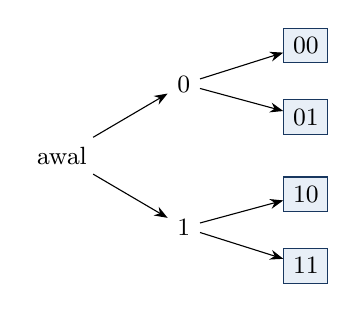
\begin{tikzpicture}[x=1.55cm,y=.70cm,>=Stealth,every node/.style={font=\small}]
\node (r) at (0,0) {awal};
\foreach \y/\m in {1.3/0,-1.3/1}{\node (b\m) at (1,\y) {$\m$};\draw[->] (r)--(b\m);}
\foreach \y/\lab/\parn in {2/00/0,.7/01/0,-.7/10/1,-2/11/1}{\node[draw=AcademicBlue,fill=SoftBlue] (s\lab) at (2,\y) {$\lab$};\draw[->] (b\parn)--(s\lab);}
\end{tikzpicture}
\end{column}
\begin{column}{.46\textwidth}
Dari setiap string panjang satu, tambahkan 0 atau 1 di kanan. Empat daun pohon adalah seluruh string panjang dua.
\[
|\{0,1\}^n|=2^n=N.
\]
Dalam urutan biner menaik, label pertama adalah $0^n$ dan label terakhir adalah $1^n$, bernilai $2^n-1$.
\end{column}\end{columns}
\bookref{hlm. 9--10; ilustrasi pendamping}
\end{frame}

\begin{frame}{Membaca tiga bit sebagai indeks basis}
\begin{center}
\begin{tabular}{ccc@{\hspace{1cm}}ccc}\toprule
String & $k$ & Basis & String & $k$ & Basis\\\midrule
000 & 0 & $e_0$ &100 &4 &$e_4$\\
001 & 1 & $e_1$ &101 &5 &$e_5$\\
010 & 2 & $e_2$ &110 &6 &$e_6$\\
011 & 3 & $e_3$ &111 &7 &$e_7$\\\bottomrule
\end{tabular}\end{center}
\textbf{Arah balik.} Untuk menulis $6$ dalam tiga bit, gunakan bobot $(4,2,1)$. Karena $6=4+2+0$, bit yang diperlukan berturut-turut adalah $1,1,0$.
\[
 e_6=(0,0,0,0,0,0,1,0)^T\quad\longleftrightarrow\quad110.
\]
Entri bernilai satu ada pada posisi ketujuh karena indeks dimulai dari nol.
\bookref{hlm. 9--10}
\end{frame}

\begin{frame}{Konkatenasi: apa yang terjadi ketika string disambung?}
Jika $x$ dan $y$ adalah string, $xy$ berarti menuliskan $y$ tepat di belakang $x$. Misalkan panjang $y$ adalah $m$.
\[
\operatorname{val}(xy)=2^m\operatorname{val}(x)+\operatorname{val}(y).
\]
Semua digit pada $x$ bergeser $m$ tempat ke kiri. Digit pada $y$ mengisi tempat yang baru tersedia.
\begin{exampleblock}{Contoh pendamping}
$x=101$, $y=01$. Karena panjang $y$ adalah dua, $xy=10101$ bernilai $4\cdot5+1=21$. Nol di depan $y$ tetap menentukan besarnya pergeseran.
\end{exampleblock}
Khusus satu bit tambahan: $x0$ bernilai $2\operatorname{val}(x)$, sedangkan $x1$ bernilai $2\operatorname{val}(x)+1$.
\bookref{hlm. 9 dan soal 2.1}
\end{frame}

\begin{frame}{String sebagai himpunan bagian}
Tetapkan himpunan dasar berurutan $(A,B,C,D)$. Bit satu berarti elemen pada posisi itu dipilih.
\begin{center}
\begin{tabular}{ccccc}\toprule
$A$ & $B$ & $C$ & $D$ & Himpunan bagian\\\midrule
0&0&0&0& $\varnothing$\\
1&0&1&0& $\{A,C\}$\\
0&1&1&1& $\{B,C,D\}$\\
1&1&1&1& $\{A,B,C,D\}$\\\bottomrule
\end{tabular}\end{center}
String $1010$ dapat berarti indeks $10$ atau himpunan $\{A,C\}$, bergantung pada keputusan pemodelan. Panjang string dan urutan elemen harus disepakati terlebih dahulu.
\bookref{hlm. 10; contoh pendamping}
\end{frame}

\begin{frame}{Penjumlahan modulo dua dan paritas}
Operasi XOR, ditulis $\oplus$, sama dengan penjumlahan modulo dua.
\[
0\oplus0=0,\quad 0\oplus1=1,\quad 1\oplus0=1,\quad 1\oplus1=0.
\]
Untuk beberapa bit, hasil XOR menyatakan apakah jumlah bit satu genap atau ganjil.
\[
1\oplus0\oplus1=0,\qquad 1\oplus1\oplus1=1.
\]
\begin{block}{Pertanyaan untuk kelas}
Jika dua bit satu ditambahkan ke deretan bit, apakah paritas berubah? Tidak: jumlah bit satu bertambah dua, sehingga sisanya modulo dua tetap sama.
\end{block}
\bookref{hlm. 10}
\end{frame}

\begin{frame}{Produk dalam Boolean: hitung irisan, lalu ambil paritas}
Untuk dua string $x,y$ dengan panjang yang sama, buku menulis
\[
x\bullet y=(x_{n-1}y_{n-1})\oplus\cdots\oplus(x_0y_0).
\]
\begin{center}
\begin{tabular}{lcccc}\toprule
Posisi dari kiri &1&2&3&4\\\midrule
$x$ &1&0&1&1\\
$y$ &1&1&0&1\\
Hasil kali per posisi &1&0&0&1\\\bottomrule
\end{tabular}\end{center}
Ada dua posisi dengan bit satu pada kedua string. Jadi $x\bullet y=(1+1)\bmod 2=0$. Hasil kali titik biasa dari kedua vektor real tersebut adalah $2$.
\bookref{hlm. 10; contoh pendamping}
\end{frame}

\begin{frame}{Dari paritas ke tanda $+1$ atau $-1$}
\begin{columns}[T]
\begin{column}{.48\textwidth}\centering
\textbf{Nilai $x\bullet y$}\\[2mm]
\begin{tabular}{c|cccc}
$x\backslash y$&00&01&10&11\\\hline
00&0&0&0&0\\01&0&1&0&1\\10&0&0&1&1\\11&0&1&1&0
\end{tabular}
\end{column}
\begin{column}{.48\textwidth}\centering
\textbf{Nilai $(-1)^{x\bullet y}$}\\[2mm]
\begin{tabular}{c|rrrr}
$x\backslash y$&00&01&10&11\\\hline
00&1&1&1&1\\01&1&$-1$&1&$-1$\\10&1&1&$-1$&$-1$\\11&1&$-1$&$-1$&1
\end{tabular}
\end{column}\end{columns}
\bigskip
\textbf{Cara membaca:} baris $11$, kolom $11$ memberi $1\oplus1=0$, sehingga tandanya $+1$. Baris $11$, kolom $10$ memberi $1\oplus0=1$, sehingga tandanya $-1$.
\par\medskip Tanda ini dapat menjadi faktor pengali amplitudo dalam transformasi kuantum. Angka pada tabel kanan belum dinormalisasi sebagai matriks uniter.
\bookref{hlm. 10 dan soal 2.3, hlm. 12}
\end{frame}

\begin{frame}{2.1 Notasi asimtotik: apa yang dianggap ukuran masukan?}
Bayangkan algoritma yang menelusuri semua string panjang $n$ satu kali. Ada $N=2^n$ string, sehingga banyak langkahnya $T(n)=2^n$ jika setiap kunjungan dihitung satu langkah.
\begin{center}\begin{tabular}{r|rrr}
$n$ (jumlah bit) &4&8&16\\\hline
$N$ (jumlah label) &16&256&65.536
\end{tabular}\end{center}
Biayanya linear terhadap $N$, tetapi eksponensial terhadap $n$. Keduanya menjelaskan algoritma yang sama.
\begin{block}{Kaitan dengan Bab 1}
Matriks operasi pada $n$ qubit berukuran $2^n\times2^n$. Menulis semua entrinya memerlukan $4^n$ tempat. Ukuran ini saja belum menentukan biaya menerapkan operasi dengan struktur khusus.
\end{block}
\bookref{pendamping \S2.1, hlm. 11--12}
\end{frame}

\begin{frame}{Contoh buku: dari jumlah persis ke suku dominan}
Pada putaran ke-$i$, algoritma menggunakan $i$ langkah. Untuk $n$ putaran:
\[
s(n)=1+2+\cdots+n=\frac{n(n+1)}2=\frac{n^2}{2}+\frac n2.
\]
Untuk melihat suku yang menentukan pertumbuhan, bagi dengan $n^2/2$:
\[
\frac{s(n)}{n^2/2}=1+\frac1n\longrightarrow1.
\]
Kita menulis $s(n)\sim n^2/2$. Artinya, rasio kedua fungsi menuju satu. Untuk $n=10$ rasionya $1{,}1$; untuk $n=100$ rasionya $1{,}01$.
\bookref{\S2.1, hlm. 11}
\end{frame}

\begin{frame}{Empat pertanyaan tentang laju pertumbuhan}
\small Untuk fungsi biaya yang akhirnya positif, gunakan definisi berikut saat $n$ cukup besar.
\begin{center}\begin{tabular}{lp{5.3cm}p{5.2cm}}\toprule
Notasi & Arti & Uji pada $s(n)=n(n+1)/2$\\\midrule
$O(g)$ & Batas atas: $s(n)\le Cg(n)$ untuk suatu $C>0$. & $s(n)=O(n^2)$, juga $O(n^3)$.\\[2mm]
$\Omega(g)$ & Batas bawah: $s(n)\ge cg(n)$ untuk suatu $c>0$. & $s(n)=\Omega(n^2)$.\\[2mm]
$\Theta(g)$ & Batas atas dan bawah berlaku untuk $g$ yang sama. & $s(n)=\Theta(n^2)$.\\[2mm]
$o(g)$ & Rasio $s(n)/g(n)$ menuju nol. & $s(n)=o(n^3)$.\\\bottomrule
\end{tabular}\end{center}
Buku juga menulis batas atas sebagai $s(n)\le Cg(n)+d$ untuk semua $n$. Untuk fungsi pembanding yang tumbuh, konstanta tambahan dapat menampung sejumlah kecil nilai awal.
\bookref{\S2.1, hlm. 11--12}
\end{frame}

\begin{frame}{Membedakan $\sim$ dan $\Theta$ melalui contoh yang sama}
Untuk $n\ge1$ berlaku
\[
\frac12 n^2\le\frac{n(n+1)}2\le n^2.
\]
Ambil $c=1/2$ dan $C=1$. Kedua batas ini membuktikan $s(n)=\Theta(n^2)$.
\[
\lim_{n\to\infty}\frac{s(n)}{n^2}=\frac12,\qquad
\lim_{n\to\infty}\frac{s(n)}{n^2/2}=1.
\]
\begin{block}{Pertanyaan diagnostik}
Apakah $s(n)\sim n^2$? Tidak. Faktor $1/2$ dapat diabaikan untuk $\Theta$, tetapi menentukan apakah dua fungsi ekuivalen secara asimtotik.
\end{block}
\bookref{\S2.1, hlm. 11--12}
\end{frame}

\begin{frame}{Logaritma, basis, dan faktor polilogaritmik}
Untuk $n>1$ dan basis logaritma tetap lebih besar dari satu,
\[
\log s(n)=2\log n+\log\!\left(\frac{1+1/n}{2}\right).
\]
Suku terakhir terbatas. Karena itu $\log s(n)=\Theta(\log n)$, dan rasio $\log s(n)/\log n$ menuju $2$.
\par\medskip
Buku memakai $\widetilde O(g(n))$ untuk menyembunyikan faktor berupa pangkat tetap dari $\log g(n)$. Misalnya,
\[
n^2(\log n)^3=\widetilde O(n^2),
\]
karena $\log(n^2)=2\log n$. Faktor logaritmik tetap ada dalam perhitungan waktu aktual.
\bookref{\S2.1, hlm. 12}
\end{frame}

\begin{frame}{Bagaimana menghitung $x^{75}\bmod M$ tanpa membentuk $x^{75}$?}
\small
Eksponen juga dapat dibaca sebagai string: $75=1001011_2=64+8+2+1$. Anggap $M\ge2$ dan $0\le x<M$.
\begin{enumerate}
\item Mulai dari $r_1=x$. Kuadratkan dan ambil sisa setiap kali:
\[
r_{2j}=r_j^2\bmod M,\qquad j=1,2,4,8,16,32.
\]
Ini menghasilkan $r_2,r_4,r_8,r_{16},r_{32},r_{64}$ melalui enam penguadratan.
\item Gabungkan hanya pangkat yang dipilih bit satu:
\[
x^{75}\bmod M=(r_{64}r_8r_2r_1)\bmod M.
\]
Kalikan dua faktor pada satu waktu, lalu segera ambil sisa.
\end{enumerate}
Total: enam penguadratan dan tiga perkalian tambahan, masing-masing diikuti reduksi modulo $M$. Sebelum setiap reduksi, kedua faktor kurang dari $M$, sehingga hasil kalinya kurang dari $M^2$.
\bookref{pembahasan soal 2.8--2.9, hlm. 13}
\end{frame}

\begin{frame}{Contoh pendamping: $3^{75}\bmod 7$}
\begin{center}\begin{tabular}{c|rrrrrrr}
$j$&1&2&4&8&16&32&64\\\hline
$r_j=3^j\bmod7$&3&2&4&2&4&2&4
\end{tabular}\end{center}
Baris kedua diperoleh berurutan: $3^2\bmod7=2$, lalu $2^2\bmod7=4$, lalu $4^2\bmod7=2$, dan seterusnya.
\begin{align*}
r_{64}r_8 &\equiv 4\cdot2\equiv1\pmod7,\\
1\cdot r_2 &\equiv 1\cdot2\equiv2\pmod7,\\
2\cdot r_1 &\equiv 2\cdot3\equiv6\pmod7.
\end{align*}
Jadi $3^{75}\bmod7=6$. Panjang representasi eksponen menentukan banyak penguadratan; biaya setiap operasi aritmetika juga bergantung pada panjang modulus.
\bookref{contoh pendamping untuk soal 2.8--2.9, hlm. 13}
\end{frame}

\begin{frame}{2.2 Latihan kelas: tiga mahasiswa, tiga cara membaca bit}
\begin{enumerate}
\item \textbf{Representasi.} String $x=011$ diulang tiga kali. Tentukan nilai $xxx$ tanpa mengembangkan sembilan bit satu per satu. Apakah hasilnya prima? Jelaskan peran nol di depan.
\item \textbf{Paritas.} Untuk $x=101$, temukan semua $y\in\{0,1\}^3$ yang memenuhi $x\bullet y=0$. Bagaimana himpunan itu berubah bila bit tengah $y$ dibalik?
\item \textbf{Biaya.} Algoritma A menyimpan satu data per string $n$ bit. Algoritma B menyimpan satu data untuk setiap pasangan posisi berbeda $i<j$. Hitung jumlah data untuk $n=8$ dan nyatakan orde pertumbuhannya terhadap $n$.
\end{enumerate}
\par\medskip Alokasi: 7 menit bekerja, 12 menit presentasi (4 menit per orang), 6 menit untuk membandingkan jawaban dan menyimpulkan. Kunci tersedia setelah slide referensi.
\bookref{latihan pendamping \S2.2, hlm. 12--13}
\end{frame}

\begin{frame}{2.3 Ringkasan: satu string, beberapa peran}
\begin{center}\begin{tabular}{lp{8.5cm}}\toprule
Saat melihat $101$ & Pertanyaan yang dapat dijawab\\\midrule
Sebagai bilangan & Berapa nilainya? $4+0+1=5$.\\[1mm]
Sebagai label basis & Komponen mana yang dibaca? $a_5$ untuk tiga qubit.\\[1mm]
Sebagai indikator & Posisi mana yang dipilih? Pertama dan ketiga.\\[1mm]
Sebagai argumen Boolean & Bagaimana paritasnya dengan $y$? $y_2\oplus y_0$.\\\bottomrule\end{tabular}\end{center}
\textbf{Jembatan ke Bab 3.} Jika $a$ adalah vektor keadaan tiga qubit, $a(101)$ dan $a(5)$ dapat merujuk ke amplitudo yang sama setelah urutan label ditetapkan. Konvensi ini juga memudahkan penamaan baris dan kolom matriks.
\bookref{\S2.3, hlm. 13; pratinjau Bab 3, hlm. 15}
\end{frame}

\begin{frame}{Referensi dan panduan membaca}
Richard J. Lipton dan Kenneth W. Regan. \textit{Quantum Algorithms via Linear Algebra: A Primer}. MIT Press, 2014. Bab 2, \textit{Numbers and Strings}, hlm. 9--13 (halaman PDF 24--28).
\begin{itemize}
\item Hlm. 9--10: bilangan, panjang string, penomoran kanonik, produk dalam Boolean, dan himpunan bagian.
\item Hlm. 11--12: notasi asimtotik dan jumlah langkah.
\item Hlm. 12--13: soal 2.1--2.9 dan ringkasan. Slide membahas pilihan soal yang menghubungkan representasi dengan biaya komputasi.
\end{itemize}
\par\medskip Untuk persiapan mengajar, ikuti contoh $101$ dari indeks basis hingga paritas; kemudian kerjakan contoh $3^{75}\bmod7$ dengan kertas sebelum menampilkan tabel.
\end{frame}

\appendix
\begin{frame}{Lampiran A: panjang string menentukan faktor pergeseran}
Untuk $x=011$, berlaku $m=3$ dan $v=\operatorname{val}(x)=3$. Setiap salinan yang digeser satu blok dikalikan $2^3=8$.
\[
\operatorname{val}(xxx)=v(2^{2m}+2^m+1)=3(64+8+1)=219.
\]
Karena $219=3\cdot73$, bilangan ini komposit. Nol di depan mempertahankan panjang blok tiga; menghapusnya dari setiap blok akan menghasilkan string berbeda, yaitu $111111$.
\begin{block}{Pengayaan soal 2.4 buku}
Untuk panjang genap $m\ge2$, $2^m\equiv1\pmod3$, sehingga $2^{2m}+2^m+1$ habis dibagi 3 dan lebih besar dari 3. Maka $xxx$ tidak prima, termasuk bila $v=0$ atau $v=1$.
\end{block}
\end{frame}

\begin{frame}{Lampiran B: membaca hasil kali Boolean sebagai syarat bit}
\[
101\bullet y=(1y_2)\oplus(0y_1)\oplus(1y_0)=y_2\oplus y_0.
\]
Nilainya nol jika dan hanya jika bit pertama dan terakhir sama. Bit tengah bebas.
\begin{center}\begin{tabular}{c|c}
$(y_2,y_0)$& Pilihan $y$\\\hline
$(0,0)$ & $000,\ 010$\\
$(1,1)$ & $101,\ 111$
\end{tabular}\end{center}
Membalik bit tengah hanya menukar dua string dalam setiap baris. Himpunan solusi tetap sama. Perhatikan bahwa sifat ini bergantung pada nol di tengah $x$.
\end{frame}

\begin{frame}{Lampiran C: menghitung objek yang benar}
\textbf{Algoritma A.} Setiap posisi memiliki dua pilihan. Maka $T_A(n)=2^n$, sehingga $T_A(8)=256$.
\par\medskip
\textbf{Algoritma B.} Posisi pertama dapat berpasangan dengan $n-1$ posisi lain di kanannya, posisi kedua dengan $n-2$, dan seterusnya:
\[
T_B(n)=(n-1)+(n-2)+\cdots+1=\frac{n(n-1)}2,\qquad T_B(8)=28.
\]
Terhadap jumlah bit, kebutuhannya masing-masing $\Theta(2^n)$ dan $\Theta(n^2)$. Jika ukuran dinyatakan sebagai $N=2^n$, kebutuhan A adalah $\Theta(N)$ dan B adalah $\Theta((\log N)^2)$.
\end{frame}
\end{document}
